\documentclass{article}
\usepackage[utf8]{inputenc}
\usepackage[a4paper, total={6in, 8in}]{geometry}

\usepackage{float}
\usepackage{physics,amssymb}
\usepackage{graphicx}
\usepackage{subfloat}
\usepackage{xcolor}   
%\usepackage{tikz}            
\usepackage{subfigure}
%\usepackage[labelformat=empty]{caption}
\usepackage{caption}
\usepackage{booktabs}
\usepackage{amsmath}
\usepackage{amsbsy}
%\usepackage{floatrow}
% Table float box with bottom caption, box width adjusted to content

%\usepackage{enumitem}
\usepackage{mathdots} % dots in matrices
\usepackage{siunitx}
\usepackage{algpseudocode} % Pseudo code
\usepackage{csquotes} % biblatex likes this
\usepackage{appendix}
\usepackage{makeidx}  % allows for indexgeneration
\usepackage{ifpdf}
\usepackage{url}
\usepackage{bigints} % the biggest of all the ints

\renewcommand{\vec}[1]{\mathbf{#1}} % bruke bold-vektorer heller enn piler
\newcommand{\vecsym}[1]{\boldsymbol{#1}} % bold-vektor for greske bokstaver og symboler
\newcommand{\uvec}[1]{\mathbf{\hat{#1}}}
\newcommand{\mean}[1]{\left < #1 \right >}
\renewcommand{\d}[2]{\frac{\partial #1}{\partial #2}}
\newcommand{\labs}[0]{\left |}
\newcommand{\rabs}[0]{\right |}
\newcommand{\figref}[2]{\ref{#1}\hyperref[#1]{.#2}}
\newcommand{\ham}{\hat{H}}
\newcommand{\tsub}[2]{#1_{\text{#2}}}
\newcommand{\inner}[2]{\bra{#1}\ket{#2}}
\DeclareMathOperator*{\E}{\mathbb{E}}

\title{Summary of STK2100}
\author{Håkon Kvernmoen}
\date{January 2021}


\begin{document}

\maketitle

\section{Regression}
\subsection{Basic Overview}
To preform a regression fit, data is needed, as well as some "target" or desired output from this data. The goal is to try to predict the target given the data. First, we record one type or multiple types of data. If we have recorded $p$ different types of data, we store these in a row vector $\Vec{x}_i = \{ x_1, ... , x_p \}$. This is a data point, located in the $p$-dimensional space of all the different things we think can predict the desired target. We also need record the target (the thing we want to model, output). This is a number $y_i$ that corresponded to the data $\Vec{x_i}$. 

One data-point is useless, so we have to record multiple different data-points as well as targets. If we have collected $n$ data-points we store these as rows in a $n \times (p+1)$ data-matrix, $\Vec{X} = (1, \Vec{x_1}, ... , \Vec{x_n})^T$. The first column is filled with ones to allow for a constant term in the model. We also need targets to each of these data-points, stored as a $n \times 1$ column vector $\Vec{y} = (y_1 , ... , y_n)^T$. 

\subsection{Linear regression}

We assume a linear relationship between the $p$ different types of data with the target. To do this we make a $(p+1) \times 1$ parameter column vector $\vecsym{\beta} = (\beta_0 , ... , \beta_p)^T$.

\begin{align*}
    \Vec{y} = \Vec{X}\vecsym{\beta} + \vecsym{\epsilon}
\end{align*}

The $\vecsym{\epsilon}$ here represents an error term, since our assumption  of a linear relationship is probably not correct and there might be noise or systematic errors in the data. Due to this error term we cannot know $\vecsym{\beta}$ exactly, so we approximate it!

\begin{align*}
    \uvec{y} = \Vec{X} \uvec{\beta}
\end{align*}

When minimizing the distance between the $\Vec{y}$ and $\uvec{y}$ points, we obtain the expression for the $\uvec{\beta}$ values corresponding to the lowest error (still assuming a linear relationship). This is called the \textit{deviance} (D), as it quantifies the discrepancy between the observed and fitted values. This is the \textit{least squares estimate}.

\begin{align*}
    D(\vecsym{\beta}) = ||\Vec{y}-\uvec{y}||^2 \Rightarrow \uvec{\beta} = (\Vec{X}^T \Vec{X})^{-1} \Vec{X}^T \Vec{y}
\end{align*}

\subsection{Regularization to Linear regression}
Linear regression is a 1-to-1 fit, and the only real constraints/modifications we can apply is removing explanatory variables or variable transformations. Two of the more common methods to en-pose stricter assumptions is \textit{Ridge} and \textit{Lasso} regression. To use these models, the explanatory variables has to be standardises. We could normalize the explanatory variables (map to [0,1]), but we want to keep model interpretability. Note that the standard is unitless.  

\begin{equation*}
    x_{stanard} = \frac{x-\mu}{\sigma}
\end{equation*}

\subsubsection{Ridge}
In ridge regression we preform ordinary linear regression with an addition to the deviance (D).  

\begin{equation*}
    D(\vecsym{\beta}, \lambda) = ||\vec{y} - \hat{\vec{y}}||^2 + \lambda ||\vecsym{\beta}||^2
\end{equation*}
With $\lambda \geq 0$, a tuning parameter where a good value is essential. The extra term here is called a shrinkage penalty and is small when the coefficients $\beta_1, ... , \beta_p$ are small. $\lambda = 0$ gives no shrinkage and we have least squares, $\lambda \rightarrow \infty$ makes all coefficients (not intercept) go towards zero. The shrinkage penalty does NOT include the intercept $\beta_0$ since we want the intercept to represent the mean of the response when $x_{i1} = x_{i2} = ... = x_{ip} = 0$.      
    
The benefit of this approach is that tough the coefficients decrease as a whole with $\lambda$, some might stay the same and some might even increase. Thus this shrinkage penalty "pulls out" the most significant coefficients while suppressing the non-significant. Bias increases with $\lambda$, but variance can decrease.       
    
\subsubsection{Lasso}
Lasso is the counter part to Ridge. One problem with Ridge is that coefficients will not directly be set to 0, but only approach it for large $\lambda$. It is thus not fit for variable selection. This is not necessarily bad for predictions (as un-significant variables will have little impact on the result), but is bad for model interpretability (especially if $p$ is large). The deviance for Lasso is

\begin{equation*}
    D(\vecsym{\beta}, \lambda) = ||\vec{y} - \hat{\vec{y}}||^2 + ||\vecsym{\beta}||_1
\end{equation*}
Again with $\lambda \geq 0$ and a good value is again essential. Where $|| \cdot ||_i$ means the sum of the absolute value, raised to the i'th power of all its components ($|| \cdot ||$ implies $\sqrt{(|| \cdot ||_{2})^2}$). 

\subsubsection{Comparing Ridge and Lasso}
Lasso has a clear advantage in that it can preform variable selection, setting some coefficients to exactly zero. This of course have limitations as, i.e. if two or more features are highly co-linear Lasso will select on of them randomly with the rest set to zero (Bad for model interpretability). In (very general) terms Ridge is best if you have a small amount of explanatory variables and/or a lot of co-linearity. Lasso shines when there  are more explanatory variables and/or where a simpler model is desired.   

\section{Classification}
\subsection{Logistic regression}
Logistic regression is kind of a classification method \textbf{and} a regression method. Pro die hard statistician's want to call it a regression, but I put it here since the goal of the method is to \textit{classify} a target. However the process of achieving the classification model, requires a \textit{regression}. If we want to preform a logistic regression on two data variables $\Vec{x} = (x_1, x_2)$ with a probability $p$ of outcome $A$. We define $\beta(x_1, x_2) = \beta_0 + \beta_1 x_1 + \beta_2 x_2$ (can of course be generalized to more)

\begin{align*}
    logit(p) = log\left(\frac{p}{1-p}\right) = \beta(x_1, x_2)
\end{align*}
where $logit$ maps the probability $p \in (0,1)$ to $logit(p) \in (-\infty, \infty)$. Solving this expression for $p$ gives.

\begin{align*}
    p(x_1, x_2) = \frac{e^{\beta(x_1,x_2)}}{e^{\beta(x_1,x_2)}+1} = \frac{1}{1+e^{-\beta(x_1,x_2)}}
\end{align*}
Now $\beta(x_1,x_2)$ can be fitted on $(-\infty, \infty)$ while the probability $p$ for outcome $A$ is still $(0,1)$. To evaluate a threshold $\mathcal{T}$ is given, typically 0.5. If the probability $p$ is bigger than the threshold, classify as A, else not A. In our example.

\begin{align*}
    \text{if } p(x_1, x_2) > \mathcal{T} \rightarrow A, \text{     else} \rightarrow \text{not } A 
\end{align*}

\subsection{Discriminant Analysis}
Using Bayes theorem, we can construct classification with more $K \geq 2$. When given the data, the goal is to somehow split the dataset with a line and project the datapoints on this line, with some criteria on how the line is drawn. 
%Discriminant analysis tries to make linear combinations of explanatory variables, so that these new linear combinations can be used for fitting instead of the original dataset. 
\subsubsection{Linear (LDA)}
Assuming that we have on explanatory variable ($p=1$) it can be shown from Bayesian statistics that we should assign $x$ to the class where $\delta_k(x)$ is largest (assuming $x$ is draw from a Gaussian distribution). The \textit{linear} comes from $\delta_k(x)$ being linear w.r.t. $x$.

\begin{align*}
    \delta_k (x) = x \cdot \frac{\mu_k}{\sigma^2} - \frac{\mu_k^2}{2\sigma^2} + log(\pi_k)
\end{align*}

Where $\mu_k$ is the mean of the $k$'th class, the variance $\sigma^2$ is assumed to be equal for all the classes and $\pi_k$ is the probability of class $k$. The LDA estimates for these are.

\begin{align*}
    \hat{\mu}_k = \frac{1}{n_k} \sum_{i:y_i=k} x_i \hspace{10px},\hspace{10px} \hat{\sigma}^2 = \frac{1}{n-K} \sum_{k=1}^{K} \sum_{i:y_i = k} (x_i-\hat{\mu}_k)^2 \hspace{10px},\hspace{10px} \hat{\pi}_k = \frac{n_k}{n}
\end{align*}
Where $i:y_i = k$ means sum over all points belonging to class $k$

This can be expanded to handle more explanatory variables ($p>1$), but dependence between variables may pose a problem. Therefore instead of $p$ Gaussian distributions, one for each variable, we rather consider a \textit{multivariate Gaussian} distribution. With a shared covariance matrix between all the classes $\vec{\Sigma}$ (a $p \times p$ matrix) and a mean for each variable $\E [\Vec{X}] = \vecsym{\mu}$ (a vector of length $p$ holding all the means for each variable) the Bayesian classifier now assigns an observation $\vec{X} = \vec{x}$ to the class where to following is highest.

\begin{align*}
    \delta_k (\vec{x}) = \vec{x}^T \vecsym{\Sigma}^{-1} \vecsym{\mu}_k - \frac{1}{2} \vecsym{\mu}_k^T \vecsym{\Sigma}^{-1} \vecsym{\mu}_k + log(\pi_k)
\end{align*}

With $\vecsym{\mu}_k$ being the mean vector of $x$ for a specific class. If $p = 2$ we do not get one decision boundary as for $p=1$, but rather 3 separating the 3 classes. These boundaries are the set of $\Vec{x}$'s where $\delta_k = \delta_l, l \neq k$ (equal propability for both classes).

\subsubsection{Quadratic (QDA)}
Instead of assuming that all the explanatory variables share the same covariance matrix, independent of class, we will now assume that each class has a specific covraiance matrix $\vecsym{\Sigma}_k$. With some data point, the Bayesian classifier assigns to the class which maximizes:

\begin{align*}
    \delta_k (\vec{x}) = - \frac{1}{2} \vec{x}^T \vecsym{\Sigma}_k^{-1} \vecsym{x} +  \vecsym{x}^T \vecsym{\Sigma}_k^{-1} \vecsym{\mu}_k - \frac{1}{2}\vecsym{\mu}_k^T \vecsym{\Sigma}^{-1} \vecsym{\mu}_k + log(\pi_k)
\end{align*}
This is \textit{quadratic} since one of the terms include $\Vec{x}$ twice.

\subsection{ROC curves}

ROC (receiver operating characteristic) curves is a graphical way to visualize how a binary (true/false) classification preforms. The $y$-axis contains the \textit{true positive rate} (TPR) and the $x$-axis the \textit{false positive rate} (FPR). These are defined as $TPR = TP/(TP+FN)$ and $FPR = TN/(TN+FP)$. The thing that varies (drawing the curve) is different thresholds $\mathcal{T}$.

\begin{minipage}{0.5\textwidth}
\begin{figure}[H]
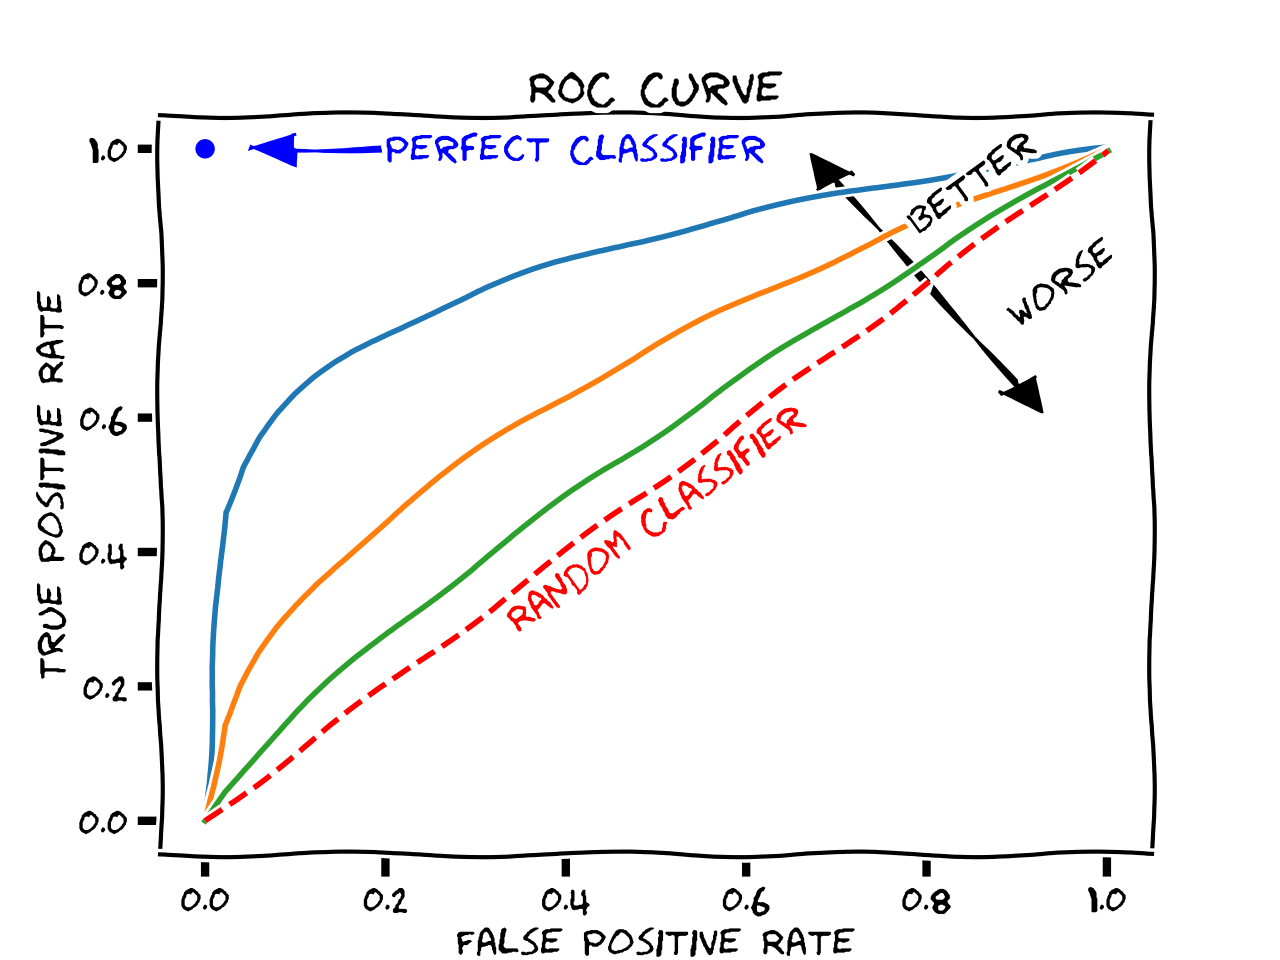
\includegraphics[width=1.1\linewidth]{roc.png}
\caption{\label{fig:roc} ROC curve}
\end{figure}
\end{minipage} \hfill
\begin{minipage}{0.5\textwidth}
An example of a ROC curve. If we were to guess 50/50 (i.e. no prediction model) our classifier would simply draw a straight line from (0,0) to (1,1). If the threshold was extremely high (very close to 1) we would have no FP (since it always guesses \textit{false}) but no TP by the same reason. Decreasing the threshold to extremely low (very close to 0) has the other effect, since it always guesses \textit{true}. If the model has any meaning full predictions the ROC curve should lay over the random classifier line. A perfect classifier would get all TP and no FP and is thus located at (0,1). 
\end{minipage}

Another measure for this is the AUC (area under curve). If $AUC = 0.5$ we have a random classifier, and $AUC = 1$ is a perfect classifier. Anything in between is expected if the model preforms meaning full predictions. 

\section{Basis functions and "Non-linear" models}

Many of these methods uses basis functions, a tool that makes classifying and distinguishing between different models easier. In general they take the form with $k$ explanatory variables.

\begin{align*}
    y_i = \beta_0 + \beta_1 b_1(x_i) + ... + \beta_k b(x_k) + \epsilon_i
\end{align*}

This is just linear regression and can easily be computed using a LS fit. The $b(\cdot)$ functions serves as some transformation of the data. For instance $b_j(x_i) = x_i^j$ is a basis function for polynomial regression. 

\subsection{Step Functions}
Step functions divides $X$ into $k$ bins with endpoints $c_1, ... , c_k$. This makes $k+1$ "categories" to place our data in, given by the $k+1$ indicator functions $C_0(X) = I(X < C_1), ..., C_j(X) = I(c_{j} < X < c_{j+1}), ... , C_k(X) = I(c_{k} \leq X)$. Essentially a data point is given a fixed value when it falls between a fixed interval. Note that $C_0(X) + ... + C_k(X) = 1$ since one of the indicator functions has to equal 1. This method is good if there are natural splits in the data, but looses a lot of data-trends. The corresponding basis function is 

\begin{align*}
    b_j(x_i) = I(c_j < x_i < c_{j+1})
\end{align*}

\subsection{Splines}
Splines depend on dividing $X$ into $k$ cuts and fitting a polynomial of degree $d$ between each cut, demanding that the $d-1$ derivative is continuous. Splines are preferred to polynomial regression since one can achieve high flexibility without high degrees.  

\subsubsection{Knot placement}

The natural approach to knot placement is to place more knots where the target is changing rapidly (to increase flexibility). In practice however, placing them uniformly often works best and is almost always done. 

Deciding the number of knots can be tricky, as too many will give too much flexibility (low bias, high variance) and too few will be too strict (high bias, low variance). Cross validation is a good option to test different values, with lets say 5-fold CV being preformed for a given amount of knots. 

\subsubsection{Cubic splines}
The most common degree is $d=3$, appropriately named \textit{cubic splines}. 

If there were no constraints, one cut would give 8 degrees of freedom for a cubic spline. Due to the constraints demanding the second derivative to be continuous we end up with 5 degrees of freedom (continuous 0'th, 1st and 2nd derivative). Thus a know only adds 1 degree of freedom and in general with $k$ cuts we have $4+k$ degrees of freedom. We often write the basis function for cubic splines as. In general for basic splines use from \texttt{gam}, \texttt{bs()}.

\begin{align*}
    h(x_i, \xi_j) = (x_i-\xi_j)^3_+ = \left\{
	\begin{array}{ll}
		(x_i-\xi_j)^3  & \mbox{if } x_i > \xi_j \\
		0 &  \text{otherwise}
	\end{array}
\right.
\end{align*}
Where $\xi_j$ is a knot. To fit a cubic spline with $k$ knots. To fit this model, one considers the constant term and (global) $X, X^2, X^3$. In addition for each knot $j = 1, ..., k$ fit $h(X, \xi_j)$, in total $4+k$ degrees of freedom. 


\subsubsection{Natural splines}
Natural splines is identical to normal splines, but we demand that the second derivative is zero at the end-points. This results in the model not going crazy for the extrapolated values at the same time not disrupting its smoothness. R comand: From \texttt{gam}, \texttt{ns()}

\subsubsection{Smoothing splines}
Smoothing splines takes a little different approach than normal splines. The goal is to minimize RSS as much as possible. The problem arises when considering the best fit is simply an interpolation of all the training data $x_1, ... , x_n$. This is of course highly overfitted, so there needs to be some sort of penalty for this high variability. One approach is find the $g$ that minimizes: 

\begin{align*}
    \sum_{i=1}^{n} (y_i-g(x_i))^2 + \lambda \int_{x_1}^{x_n} g''(t)^2 dt
\end{align*}

This is simply normal RSS, with an additional integral over the second derivative of $g$ (over the whole data set), with $\lambda$ being a tuning parameter. This takes the form of a "Loss+Penalty" formulation. The second derivative represents the \textit{roughness} of the function. The function $g$ is squared to not discriminate against negative concave functions and the integral sums over the whole data-range. It can be shown that this represents a natural cubic spline with knots at $x_1, ... , x_n$ with an additional penalty demanding that the function should be smooth.   

With $\lambda = 0$ there will be no roughness penalty and the points $x_1, ... , x_n$ will be exactly interpolated. With $\lambda \rightarrow \infty$ the fit will be perfectly smooth and just be a straight line (equal to the normal LS fit). Thus the \textit{effective degrees of freedom} decreases from $[n,2)$ with $\lambda \in [0, \infty)$. We do not need to choose the location of the knots as with normal splines or natural splines, but a good $\lambda$ is needed. This can be done with CV, but there is a closed formed solution for LOOCV.

\begin{align*}
    RSS_{LOOCV}(\lambda) = \sum_{i=1}^n \left( y_i - \hat{g}_\lambda^{(-i)} (x_i)\right)^2 = \sum_{i=1}^n \left( \frac{y_i - \hat{g}_\lambda (x_i)}{1-[\vec{S_\lambda}]_{ii} } \right)^2
\end{align*}
$\hat{g}_\lambda^{(-i)}$ is the fit of $g$ using all the data except $i$, then evaluated at $i$. Where $\vec{S}_\lambda$ is the solution to $\hat{\Vec{g}}_\lambda = \Vec{S}_\lambda \Vec{y}$. $\Vec{S}_\lambda$ is statistically difficult, but there is a formula for this (INSERT R COMMAND HERE). In addition the effective degrees of freedom are $df_\lambda = Tr(\Vec{S}_\lambda)$.  R command from \texttt{gam}, \texttt{s()}

\subsection{Generalized Additive Models (GAMs)}
GAMs is a natural extension of linear regression. To allow for non-linear relationships between the explanatory variables, each component is modeled by a smooth non-linear functions $f(\vec{x}_j)$. It is important that these function still are \textit{additive} such that the response $\vec{y}$ can be expressed as a sum of these non-linear functions. The Model then becomes.

\begin{align*}
    y_i = \beta_0 + \sum_{i=1}^{p} f_j (x_{ij}) + \epsilon_i
\end{align*}

\begin{itemize}
    \item Pros
    \begin{enumerate}
        \item Since $f_j$ is non-linear, we do not need to manually try different transformations of $X_j$ as we need in a linear regression setting
        \item Since we still have a additive model, investigating the effect of variable $X_j$ on the response $Y$ is easy, no loss of interpretability.
        \item The smoothness of $f_j$ can be summarized via degrees of freedom
    \end{enumerate}
    \item Cons
    \begin{enumerate}
        \item Since the model is restricted to be additive, interacting terms of the form $X_j \times X_k$ are still missed if they are not explicitly included. 
    \end{enumerate}
\end{itemize}

In the \texttt{gam} library the \texttt{gam} function allows for GAM fits. \texttt{s(variable, degree)} fits smoothing splines

\section{Tree-based Methods}
These methods are based on segmenting the predictor space into a number of simpler regions. The rules for the segmentation are summarized in a decision tree giving the name tree-based methods. They can be applied to both regression and classification.
Each region is called a \textit{terminal node}. Where the split happens is called  a \textit{internal node}, opening up two new \textit{branches}.

\subsection{Regression}
When building a regression tree there are two main steps.

\begin{enumerate}
    \item Use all the features $\vec{x}_1, ... , \vec{x}_p$ to divide the data into $J$ non-overlapping regions $R_1 , ... , R_J$.
    \item When predicting using a new data point $\vec{x}_k$ use the decision tree to find the right regions $R_j$. The predicted value will be the mean of all the training data points belonging to region $R_j$
\end{enumerate}

Step 1 can be done multiple different ways, but a common approach is to divide the regions using hyper-cubes (rectangles for two explanatory variables, cubes for three) that minimizes the $RSS$.
\begin{align*}
    RSS = \sum_{j=1}^{J} \sum_{i \in R_j} (y_i - \hat{y}_i)^2
\end{align*}
A common top-down (starting from the top), greedy (best split is done at a particular step, not looking forward for better splits) approach called \textit{recursive binary splitting}. This is very computationally expensive. Starting at the top, for each explanatory variables $x_j$  propose an \textit{internal node} with the cut point $s$. It then makes a split into to regions corresponding the.

\begin{align*}
    R_1(j,s) = \{ x | x_j < s \} \text{ and } R_2(j,s) = \{ x | x_j \geq s \}
\end{align*}
And choose the $j,s$ combination that minimizes $RSS$. That is minimizes ($\hat{y}_{R_1}, \hat{y}_{R_2}$ are the means of the traning observations in $R_1(j,s), R_2(j,s)$). Repeat this at each new \textit{branch} and continue until we have a pre-set number of $J$ \textit{terminal nodes} (regions) or another stopping criteria such as maximum $n$ number of observations for each region. Surprisingly this can be done quite quickly is $p$ is not too large and $J$ is not stupidly large.

\begin{align*}
    \sum_{i: x_i \in R_1} (y_i -\hat{y}_{R_1})^2 + \sum_{i: x_i \in R_2} (y_i -\hat{y}_{R_2})^2 
\end{align*}

\subsection{Classification}
Classification trees are very similar to regression trees, however instead of predicting a value based one the mean in each region, we instead classify to the class containing most instances in each region. In addition we can not use RSS, as it does not have any significant meaning in classification. A natural choice would be the \textit{classification error rate}, the fraction of training observations in each region that to not belong to the most common class. This is often not sufficiently sensitive, and to other measures of region "purity" is often prefred. The \textit{Gini index} and \textit{cross-entropy}.

\begin{align*}
\textit{Gini index: } G &= \sum_{k = 1}^{K} \hat{p}_{mk} (1-\hat{p}_{mk}) \\
\textit{Cross-entropy: } D &= -\sum_{k}^{K} \hat{p}_{mk} \log{\hat{p}_{mk}}
\end{align*}

Where $\hat{p}_{mk}$ is the proportion of the observations from the $m$th region that are from the $k$th class. The gini index is small if $\hat{p}_{mk} \approx 1$ or $\hat{p}_{mk} \approx 0$. Thus if a region contains a lot of instances of the same class ($\hat{p}_{mk} \approx 1$) or very few instances of the same class ($\hat{p}_{mk} \approx 0$) the Gini index will report a small error. The same follows for the cross-entropy ($log(1) = 0$) and the minus sign is there since $0 \leq \hat{p}_{mk} \leq 1 \rightarrow \log(\hat{p}_{mk}) \leq 0$. Both these measures takes on small values if the region is \textit{pure}.  

\subsection{Tree Pruning}
If the amount of regions are large, this is prone to over fitting. One can of course decrease the number of regions $J$ or set a $RSS$-decrease threshold for each split. Even tough this will result in smaller trees, one can fall into the trap where one misses a seemingly useless split early on that turns out to reduce $RSS$ by a lot later down the tree. A better candidate is \textit{cost complexity pruning}/\textit{weakest link pruning} (a rose by any other name would smell as sweet). We begin by growing a very large tree $T_0$. We want to check different $MSE$ of sub-trees of $T_0$, but of course the amount of combinations are ridiculously large. By considering a sub-tree with $T$ \textit{terminal nodes} and a non-negative tuning parameter $\alpha$. For different alpha's we train.

\begin{align*}
    \sum_{m=1}^{T}\sum_{x_i \in R:m} (y_i - \hat{y}_{R_m})^2 + \alpha T
\end{align*}
$\alpha = 0$ leaves us (pun intended) with the un-pruned tree $T_0$ and increasing $\alpha$ penalises the tree for having a lot of branches. Now that we have trees for different amount of leaves one can use k-fold CV to plot the $MSE$ against the number of \textit{external nodes}.

\subsection{Bagging}
In general tree based methods suffer from high variance. This means that if we train 100 different trees of 100 different subsets of a data set, the models might look very different. To reduce the high variance, a technique called \textit{bagging} is often applied.
\\
The idea of bagging is to pick $B$ number of subset from the original data. For each $B$, we train a deep tree model $\hat{f}_b(x)$. Finally we average over all $\hat{f}_b(x)$ to achieve our final model.

\begin{align*}
    \hat{f}_{bag} (x)= \sum_{b=1}^{B} \hat{f}_b (x)
\end{align*}

Since each tree is grown deep, the individual trees have a high variance but low bias. Averaging over many trees aims to reduce the variance. For regression one simply averages over the predicted target $\hat{y}$ to find the bag target. Classification on the other, might use something like \textit{majority vote}, the target that has the most trees classify to its class is chosen. The choice of large $B$'s often does not lead to over fitting. One can chose a high enough $B$ such that the train error stabilizes.  

\subsubsection{Out-of-Bag error estimation (OOB error)}
In stead of using CV or validation sets to evaluate the test error of a bagged tree, one can use the OOB error. For $n$ data points pick out $n$ randomly (allowing for picking the same point more than once). On average this chooses $1-e^{-1} \approx 2/3$ of the data points. For each tree one can use the remaining $1/3$ points to produce the test error. For the $i$th OOB observation one can average over all the predictions (regression) or majority vote (classification). This is a good choice when cross-validation is too computationally expensive.

\subsubsection{Variable Importance Measures}
Since we have a $B$ trees, we loose a lot of interpretability. One can iterate over all $B$ trees and for each variable split, record the \textit{decrease} in RSS or Gini index. The total amount can then be displayed for each variable giving some hints to what variables are important for the collection of trees.

\begin{itemize}
    \item Pros
    \begin{enumerate}
        \item Bagging typically results in improved accuracy over predictions using a single tree \item Can evaluate test error using OOB error estimation. No need for CV  
        \item Using variable importance one can "regain" some of the lost interpretability. 
    \end{enumerate}
    \item Cons
    \begin{enumerate}
        \item Since there are a lot of trees that average/vote for (regression/classification) a prediction, we loose a lot of the interpretability inherent in the tree model.  
    \end{enumerate}
\end{itemize}

\subsection{Random Forest}
In bagging the $B$ trees are somewhat correlated. Since at every split all trees considers all the $p$ predictors to decrease RSS/Gini index the trees might look very similar. Random forest tries to \textit{decorrelate} the trees, by limiting the amount of possible variables to split. At each split a random sample of $m > p$ possible predictors are chosen. Commonly $m = \sqrt{p}$ is chosen, but can be varied to optimize performance, $m = p$ reduces to bagging. 
\\
This is (counter-intuitively) often a good choice since a strong predictor at the top of the tree will produce similar trees if all $p$ predictors are considered. Limiting the choice to $m$ predictors for each split motivates more diverse trees. As in bagging large $B$s does not overfit and can be chosen large enough for test error to stabilize.   

\section{Support Vector Machines}
Support vector machines is a loose term containing three models. All the methods are used for \textit{classification} 

\begin{enumerate}
    \item Maximal margin classifier
    \item Support vector classifier 
    \item Support vector machine
\end{enumerate}

\subsection{Maximal margin classifier}
For a binary classification (2 targets, true/false situation) we try to split the features space using a \textit{hyperplane}. A hyperplane is a flat $p-1$ dimensional affine (it dose not need to pass the origin) subspace of a $p$ dimensional feature space. $p=2$ gives a line, $p=3$ gives a plane and so on. Given a data point (column vector) $x_i = (x_{i1}, x_{i2}, ... , x_{ip})$ the hyperplane can be drawn by the line.

\begin{align*}
     f(x_i) = \beta_0 + x_i^T \beta \hspace{10px}\text{plane at } f(x_i) = 0
\end{align*}
For a new data-point $x_j$ it can be classified to two different classes $\hat{y}_j = \{-1, 1\}$ by. 
\begin{align*}
    f(x_j) = \begin{cases}
    f(x_j) > 0 & \hat{y}_j = 1 \\
    f(x_j) < 0 & \hat{y}_j = -1
    \end{cases}
\end{align*}
The magnitude of $|f(x_j)|$ can be used to decide how "sure" the classifier is about the class. Thus $|f(x_j)| >> 0$ means we are very sure and $|f(x_j)| \approx 0$ means we are not. There is actually an infinite amount of possible planes, as very tiny rotations/translations of $f(x)$ can still divide the two classes. To pick the "best" plane one finds the plane that has the largest margin. With the margin as $M$ one tries:

\begin{align*}
    \underset{\beta}{\text{Max }} M \hspace{20px}\text{with} \hspace{20px}\sum_{j=1}^{p} \beta_i^2 = 1 \hspace{20px}\text{such that}\hspace{20px}f(x_i, \beta) \geq M
\end{align*}
To read this one can go backwards. The last function $f(x_i, \beta) \geq M$ means that if $x_i$ belongs to class $1$ the point will be on the right side of the plane $f(x_i, \beta) > 0$ and have at least the distance $M$ ($f(x_i, \beta) \geq M$) from the plane, with negative sign for class $-1$. This should hold for all $i = 1, ... , n$. The constraint on the $\beta$'s ensures the $f(x_i, \beta)$ is the distance from the hyperplane to the observation. Lastly we find this margin $M$ with varying the hyperplane trough the $\beta$'s. 
 
\subsection{Support Vector Classifier}
To draw a hyperplane splitting the two classes is of course not always possible. In the cases that we can draw a hyperplane, we often don't want to draw a margin that exactly splits the training data. Such a margin is very sensitive to points close to the margin, thus the decision boundary can by extremely influenced by one point (resulting in overfitting). We now allow some points to be inside the margin (\textit{soft-margin classifier}) and even on the wrong side of the hyperplane.

This is done by adding a \textit{slack variable} $\epsilon = \epsilon_1, ... , \epsilon_n$ to each of the training data-points. These are also tweaked to find the optimal $M$ such that we now have $n+p$ parameters to tweak. The optimization is identical to the maximal margin classifier but with the modification:

\begin{align*}
    f(x_i, \beta) \geq M(1-\epsilon_i) \hspace{20px}\text{with every } \epsilon_i \geq 0 \hspace{20px}\text{such that}\hspace{20px}\sum_{i=1}^{n}\epsilon_i \leq C
\end{align*}
Where $C$ is a positive tuning parameter. Classification is equal to the maximal margin classifier, assign class according to which side of the hyperplane $x_j$ is located. $C$ is a budget. Larger $C$ means more freedom to violate the margin (or even hyperplane). If $\epsilon_i > 0$ the margin is violated and if $\epsilon_i > 1$ then $x_i$ is on the wrong side of the hyperplane. $C > 0$ means that a maximum of $C$ observations are located on the wrong side of the hyperplane. The margin $M$ tends to grow with the value of $C$. In the optimization in turns out that only the observations directly on or in violation of the margin (\textit{support-vectors}) influences the classifier. With a high $C$ and thus a high margin, many observations violate the margin and thus we have a low variance but potentially high bias. The opposite is true for a small $C$.

\subsection{Support Vector Machine}
Support vector machines (SVM) tries to deal with non-linear boundaries. There are many different ways to do this. The most obvious solution is to make new observations by interaction terms, higher order polynomials or special function with the old observation. The problem with this is that the solution space will be enlarged and can result in very costly computations.  

Instead of increasing the observation space, SVM obtains non-linear boundaries by the use of \textit{kernals}. A kernal defines a new inner product. It turns out that the solution to the support vector classifier only involes inner products between the support vectors. Let $\mathcal{S}$ hold the indicies on the support vectors. Then any solution can be written as the function:

\begin{align*}
    f(x) = \beta_0 + \sum_{i \in \mathcal{S}} \alpha_i K(x, x_i)
\end{align*}

Where $K$ is the kernal, defining the inner product. It can take many forms, a few of them are:

\begin{itemize}
    \item Linear: $K(x_i, x_j) = \sum_{k=1}^{p} x_{ik}x_{jk}$. This is a support vector classifier
    \item Polynomial: $K(x_i, x_j) \left( 1+ \sum_{k=1}^{p} x_{ik}x_{jk}\right)^d, d > 1$
    \item Radial: $K(x_i, x_j) = exp(-\gamma \sum_{k=1}^{p}(x_{ik}-x_{jk})^2), \gamma > 0$
\end{itemize}
\section{Potential pitfalls}
\subsection{Overfitting}
Considering the MSE $ = \E[\uvec{y}-f(\Vec{x})]$ where $f(\Vec{x})$ represents the target (real, but unknown) function. This quantity can be interpreted as.

\begin{align*}
    MSE = \E[\uvec{y}-f(\Vec{x})] = \text{bias}^2 + \text{variance} + \text{irreducible}
\end{align*}

\begin{table}[H]
    \centering
    \begin{tabular}{|c|c|c|}
         \hline
         Type &  High & low\\
         \hline
         Bias & Strict model, a lot of assumptions & Flexible model, few assumptions \\
         \hline
         Variance & New data preforms bad, overfitting & New data preforms well \\
         \hline
         Irreducible & Lots of noise from data &  Little noise from data\\
         \hline
    \end{tabular}
    \caption{Caption}
    \label{tab:my_label}
\end{table}

\section{Data-set splitting}
Fitting all the data to a model is in general a bad approach, as the model can be \textit{overfitted} for flexible models and/or makes testing the accuracy of the model infeasible (the model is bias to the sample). 

\subsection{Test/train split}
This approach simply splits the data set into a train and test set. The exact split is dependent on many factors, but normally something like 2/3 train and 1/3 test is used. The model is fitted on the training data, and selection of which model to use/evaluation of the accuracy is chosen trough predictions using the test set. To make the train/test split as un-biased as possible, random selection is preferred (the data can somehow be structured).

\begin{itemize}
    \item Pros 
    \begin{enumerate}
        \item Very computationally cheap, pretty much the "simplest" thing to do
        \item Provides more precise results than fitting with all the data despite not being computationally expensive
    \end{enumerate}
    
    \item Cons
    \begin{enumerate}
        \item If many models are tested and the test set is used to pick the best model, the model can be biased towards the test set. Sometimes a third split is made (validation set) to reduce this bias.
        \item The number of samples to preform the fit are reduced, can in turn increase error.
        \item Not stable results, can depend on the randomly chosen train/test split.
    \end{enumerate}
\end{itemize}

\subsection{Cross Validation}
Cross validation (CV) is based on splitting the data into different \textit{folds} (parts) and training the model one some folds, while testing on others, repeated many times to make averages of RSS, MSE, ... 

\begin{itemize}
    \item Pros
    \begin{enumerate}
        \item More stable than Train/Test
        \item Reflects the population better than train/test
    \end{enumerate}
    
    \item Cons
    \begin{enumerate}
        \item More computationally expensive than train/test (tough often doable is if $k \approx 5-10$)
        \item Can produce some instability, folds are selected randomly 
    \end{enumerate}
\end{itemize}

\subsection{Leave-one-out CV (LOOCV)}
Pick on data point. Train the model on every other data point, and evaluate on that chosen point. Reapeat for all points

\begin{itemize}
    \item Pros
    \begin{enumerate}
        \item Very low bias, model is trained on the whole data-set
        \item Do not overestimate test error
        \item Zero randomness, stable results
    \end{enumerate}
    \item Cons
        \begin{enumerate}
            \item VERY computationally expensive. Especially for large $n$ and EXTREMELY if model takes a long time to train. 
        \end{enumerate}
\end{itemize}

LOOCV is pretty much never feasible to do, but for ordinary LS (No Ridge/Lasso) there is a closed form solution.

\begin{align*}
    MSE = \frac{1}{n} \sum_{i=1}^{n} \left( \frac{y_i - \hat{y}_i}{1 - h_i} \right)^2 \hspace{20px} h_i = \frac{1}{n} + \frac{(x_i-\E[{x}])^2}{\sum_{i'=1}^{n} (x_{i'}-\E[{x}])^2}
\end{align*}


\section{Analysis}
 

\section{Model Selection}
All selection models can use different measures to classify the "best" model or "smallest" error. Some examples:

\begin{itemize}
    \item Complexity-indipendent: MSE, RSS, $R^2$
    \item Complexity-dependent: AIC, BIC, adjsted $R^2$
\end{itemize}


\subsection{Best Subset Selection}
With $p$ features try all $2^p$ model and use the one with the smallest error. Very good but stupidly expensive, especially if model takes a long time to train. Large $p$ makes this infeasible. Often models are trained on the training data, and the $p+1$ lowest RSS/$R^2$ models are chosen. Then some CV scheme is used to choose which of these models to use with some complexity penalising measure (to reduce overfitting). All in all conceptually appealing but computationally infeasible. 

\subsection{Stepwise Selection}
\subsubsection{Forward and backward}
Start with constant term. For $k = 0, ... , p-1$ try all $p-k$ models and save the best model for each $k$. Then select a single model from these using some complexity-dependent measure. Results in a total number of models:

\begin{equation*}
    1 + \sum_{k=0}^{p-1} (p-k) = 1 + \frac{p(p+1)}{2} 
\end{equation*}

More computationally feasible than Best Subset. Works well in practice, but not guaranteed to find the best possible model of the $2^p$ possibilities. Similarly one can use backward selection. Totally identical but start with $p$ predictors and remove one at a time. Forward selection works for (Assuming LS) $p > n$ as a maximum of $n$ features can be chosen, but backward selection can NOT do this.

\section{Special functions and (some) needed statistics}
\subsection{Some error analysis}
There are a few assumptions about the errors that we (almost always) make to preform error analysis.

\begin{enumerate}
    \item Independent variable(s) measured without uncertainty (the $\Vec{X}$ data). Almost always false but always assumed.
    \item Errors are normally distributed $N\sim(0,\sigma^2)$
    \item Constant $\sigma^2$ 
    \item Errors are independent, $e_i$ does not effect $e_j$ 
\end{enumerate}
Quantifying this error, we define the \textit{residual} of the $i$th data point $e_i = y_i-\hat{y}_i$. We are mostly interested in the global error, so we define the residual sum of squares (RSS) as:

\begin{align*}
    RSS = \sum_{i=1}^{n} e_i^2
\end{align*}
The \textit{root square error} (RSE). Provides an absolute measure of lack of fit of the model to the data.

\begin{align*}
    RSE = \sqrt{\frac{RSS}{n-p-1}}
\end{align*}
And the \textit{total sum of squares} (TSS)

\begin{align*}
    TSS = \sum_{i=0}^{n} = (y_i - \Bar{y})^2
\end{align*}
We also define $R^2$ as a mesure of how good a linear fit our model is. Note that $R^2$ will \textbf{always} increase (or stay the same) when adding more paramters $p$ as we fit the data set better, but this might not reflect the true population and might preform worse on new test data. Adjusted $R^2$ tries to compensate for this.

\begin{align*}
    R^2 = 1 - \frac{RSS}{TSS}
\end{align*}

When comparing models the response should ideally be on the original scale of the data. You can compear models with the same target transformation, but not when they differ.

\subsection{Likelihood function}
Often just called likelihood describes how "good" a fit is as a function of parameters $\vecsym{\theta}$. It is for by assuming that both the input variables $\Vec{X}$ \textit{and} output variables $\Vec{Y}$ comes from a join probability distribution. It is viewed as a function of $\vecsym{\theta}$ only, so the recorded data ($\Vec{x} \text{ and } \Vec{y}$) are viewed as constant. This is often written as 

\begin{align*}
    L(\Vec{y}|\vecsym{\theta}) = p_{\theta}(\Vec{y}) = P_{\theta}(\Vec{Y}=\Vec{y})
\end{align*}

Meaning the likelihood of the outcome $\Vec{y}$ (sampled from the random variable $\Vec{Y}$), as a function of $\vecsym{\theta}$. We say that the $\uvec{\theta}$ that maximizes $L$, is the maximum likelihood estimate (MLE). 

The data is assumed to be collected from a pdf/pmf $q$. If we have $n$ data points $x_1, ... , x_n$ these are sampled with a given parameters $\theta$. That is, they are sampled from $q(x|\theta)$.
 
\subsubsection{Indicator Variables}
If we have a qualitative (non-continuous, often not numerical) variable we have to apply indicator functions. If we add $k$ indicator functions, we expand our data-matrix $\Vec{X}$ with $k$ new columns, and $\uvec{\beta}$ we $k$ new entries respectively. This is normally represented by the function $I_i$ corresponding to one of the $k$ qualitative variables. If the qualitative variable is "male" or "female", the form of $I_M$ might look like. 

\begin{align*}
I_M = 
\left\{
	\begin{array}{ll}
		1  & \mbox{if } \text{"male"} \\
		0 & \mbox{if } \text{"female"}
	\end{array}
\right.
\end{align*}

We now have to make model for "female", such that $I_M = 0$ gives expected results. The parameter $\beta_i$ corresponding to "male" should be the average difference between "male" and "female" in our model, such that in case the data point is "male" our model will compensate for this. 

\subsubsection{Variable Transformations}
The data has to be linear with respect to the parameter, but we can still use non-linear variables as out data. We can apply how as many transformations as we want, i.e. $X = (1, x_1, x_2, x_2/x_1, e^{(x_2^2 - x_1)})$. A common variant is the polynomial model $X = (1, x_1, x_2^2 , ... , x_n^p)$. We can also transform the target.

\end{document}


